\begin{tikzpicture}
	\pgfplotsset{/tikz/font={\small}}
	\begin{axis}[
		grid=both,
		width=1.0\textwidth,
		height=0.3\textheight,
		x tick label style={
		/pgf/number format/1000 sep=},
		ytick={0,...,-7},
		y tick label style={
			/pgf/number format/.cd,
			fixed,
			fixed zerofill,
			precision=1,
		},
		y dir=reverse,
		ymax=1, ymin=-7,
		ylabel={Y BD-rate (\%)},
		% enlargelimits=0.15,
		enlarge y limits=false,
		enlarge x limits=0.04,
		legend style={at={(0.5,-0.45)},
		anchor=north,legend columns=-1},
		ybar interval,
		% bar width=1pt,
		xtick=data,
		xtick align=inside,
		% nodes near coords,
		% xlabel={Sequences},
		% xlabel near ticks,
		symbolic x coords={
			NebutaFestival,
			PeopleOnStreet,
			SteamLocTrain,
			Traffic,
			BasketballDrive,
			BQTerrace,
			Cactus,
			Kimono1,
			ParkScene,
			BasketballDrill,
			BQMall,
			PartyScene,
			RaceHorses\_480p,
			BasketballPass,
			BlowingBubbles,
			BQSquare,
			RaceHorses\_240p,
			FourPeople,
			Johnny,
			KristenAndSara,
			BasketDrillText,
			ChinaSpeed,
			SlideEditing,
			SlideShow,
			Overall,
		},
		x tick label style={rotate=-60,anchor=west},
		]

		\addlegendentry{Sep KLT RA}
		\addplot coordinates {
		(NebutaFestival,   -0.08)
		(PeopleOnStreet,   -0.45)
		(SteamLocTrain,     0.03)
		(Traffic,          -0.58)
		(BasketballDrive,  -0.25)
		(BQTerrace,        -0.05)
		(Cactus,           -0.34)
		(Kimono1,          -0.03)
		(ParkScene,        -0.58)
		(BasketballDrill,  -0.55)
		(BQMall,            0.12)
		(PartyScene,       -0.07)
		(RaceHorses\_480p, -0.40)
		(BasketballPass,   -0.12)
		(BlowingBubbles,   -0.07)
		(BQSquare,          0.08)
		(RaceHorses\_240p, -0.34)
		(FourPeople,       -0.59)
		(Johnny,           -0.12)
		(KristenAndSara,   -0.12)
		(BasketDrillText,  -0.48)
		(ChinaSpeed,        0.17)
		(SlideEditing,      0.52)
		(SlideShow,         0.50)
		(Overall,          -0.16)
		};

		\addlegendentry{Sep RDOT RA}
		\addplot coordinates {
		(NebutaFestival,   -0.05)
		(PeopleOnStreet,   -0.52)
		(SteamLocTrain,     0.00)
		(Traffic,          -0.91)
		(BasketballDrive,  -0.42)
		(BQTerrace,        -0.63)
		(Cactus,           -0.78)
		(Kimono1,          -0.21)
		(ParkScene,        -0.72)
		(BasketballDrill,  -0.94)
		(BQMall,           -0.58)
		(PartyScene,       -0.68)
		(RaceHorses\_480p, -0.58)
		(BasketballPass,   -0.52)
		(BlowingBubbles,   -0.52)
		(BQSquare,         -0.53)
		(RaceHorses\_240p, -0.43)
		(FourPeople,       -1.23)
		(Johnny,           -0.78)
		(KristenAndSara,   -0.73)
		(BasketDrillText,  -0.88)
		(ChinaSpeed,       -0.43)
		(SlideEditing,     -0.76)
		(SlideShow,        -0.53)
		(Overall,          -0.60)
		};

		\addlegendentry{N-sep KLT RA}
		\addplot coordinates {
		(NebutaFestival,   -0.08)
		(PeopleOnStreet,   -1.14)
		(SteamLocTrain,    -0.11)
		(Traffic,          -1.47)
		(BasketballDrive,  -1.24)
		(BQTerrace,        -1.28)
		(Cactus,           -1.19)
		(Kimono1,          -0.31)
		(ParkScene,        -0.91)
		(BasketballDrill,  -3.79)
		(BQMall,           -0.33)
		(PartyScene,       -0.74)
		(RaceHorses\_480p, -1.42)
		(BasketballPass,   -0.96)
		(BlowingBubbles,   -0.93)
		(BQSquare,         -0.24)
		(RaceHorses\_240p, -1.40)
		(FourPeople,       -1.52)
		(Johnny,           -0.97)
		(KristenAndSara,   -0.94)
		(BasketDrillText,  -3.15)
		(ChinaSpeed,       -0.08)
		(SlideEditing,      0.77)
		(SlideShow,         0.23)
		(Overall,          -0.97)
		};

		\addlegendentry{N-sep RDOT RA}
		\addplot coordinates {
		(NebutaFestival,   -0.11)
		(PeopleOnStreet,   -1.11)
		(SteamLocTrain,    -0.30)
		(Traffic,          -1.96)
		(BasketballDrive,  -1.85)
		(BQTerrace,        -2.45)
		(Cactus,           -2.16)
		(Kimono1,          -0.48)
		(ParkScene,        -1.23)
		(BasketballDrill,  -6.34)
		(BQMall,           -1.47)
		(PartyScene,       -1.75)
		(RaceHorses\_480p, -1.97)
		(BasketballPass,   -1.78)
		(BlowingBubbles,   -1.90)
		(BQSquare,         -1.40)
		(RaceHorses\_240p, -1.84)
		(FourPeople,       -2.54)
		(Johnny,           -2.37)
		(KristenAndSara,   -2.50)
		(BasketDrillText,  -5.57)
		(ChinaSpeed,       -0.95)
		(SlideEditing,     -0.76)
		(SlideShow,        -1.55)
		(Overall,          -1.93)
		};

	\end{axis}
\end{tikzpicture}
